\documentclass[en]{../../../../../../eplexam}

\hypertitle{sigsys-FSAB1106}{4}{FSAB}{1106}{2014}{Juin}
{Louis Devillez}
{Luc Vandendorpe et Vincent Wertz}

\section{Question 1}
On considère le système causal représenté à la figure suivante:
\begin{center}
	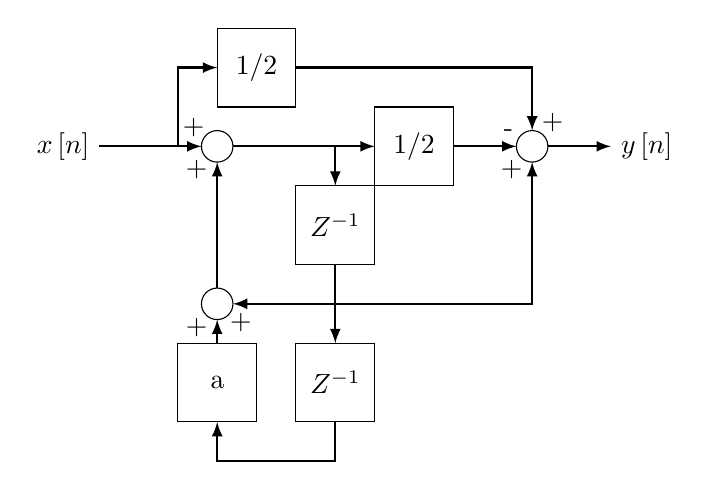
\begin{tikzpicture}
		\draw (-0.5,0) node[left]{$x\left[n\right]$} [thick,-latex] --(0.8,0);
		\draw (0.7,0)node[above]{+};
		\draw (1,0) circle(0.2);
		\draw [thick,-latex] (0.5,0) -- (0.5,1) -- (1,1);
		\draw (1,1.5) rectangle (2,0.5);
		\draw (1.5,1) node[]{1/2};
		\draw [thick,-latex](1.2,0) -- (2.5,0) -- (2.5,-0.5);
		\draw [thick,-latex](2.5,0) -- (3,0);
		\draw (3,0.5) rectangle (4,-0.5);
		\draw (3.5,0)node[]{1/2};
		\draw [thick,-latex](4,0) --(4.8,0);
		\draw (4.7,0)node[above]{-};
		\draw [thick,-latex] (2,1) -- (5,1) -- (5,0.2);
		\draw (5,0.3)node[right]{+};
		\draw (5,0) circle(0.2);
		\draw (2,-0.5) rectangle (3,-1.5);
		\draw (2.5,-1)node[]{$Z^{-1}$}; 
		\draw [thick,-latex](2.5,-1.5) -- (2.5,-2) -- (1.2,-2);
		\draw (1.3,-2)node[below]{+};
		\draw (1,-2) circle(0.2);
		\draw [thick,-latex] (1,-1.8) -- (1,-0.2);
		\draw (1,-0.3) node[left]{+};
		\draw [thick,-latex] (2.5,-2) -- (2.5,-2.5);
		\draw (2,-2.5) rectangle (3,-3.5);
		\draw (2.5,-3) node[]{$Z^{-1}$};
		\draw [thick,-latex] (2.5,-3.5) -- (2.5,-4) -- (1,-4) -- (1,-3.5);
		\draw (0.5,-3.5) rectangle (1.5,-2.5);
		\draw (1,-3) node[]{a};
		\draw [thick,-latex](1,-2.5) -- (1,-2.2);
		\draw (1,-2.3) node[left]{+};
		\draw [thick,-latex](2.5,-2) -- (5,-2) -- (5,-0.2);
		\draw (5,-0.3)node[left]{+};
		\draw [thick,-latex] (5.2,0) -- (6,0)node[right]{$y\left[n\right]$};
	\end{tikzpicture}
\end{center}
\begin{itemize}
	\item Déterminer une représentation d'état du système
	\item Calculer la fonction de transfert associée
	\item Étudier la stabilité interne du système pour les mêmes valeurs du paramètre $a=0$, $a=1$ et $a=2$
	\item Étudiez la stabilité BIBO du système pour les mêmes valeurs du paramètre a
	\item Définir en quelques lignes la notion de commandabilité d'un système linéaire
	\item Étudiez la commandabilité et l'observabilité du système pour les trois valeurs du paramètre a mentionnées plus haut
\end{itemize}

\begin{solution}
	\begin{itemize}
		\item Représentation d'état:	$$
		\begin{bmatrix}
		q_1\left[n+1\right]\\
		q_2\left[n+1\right] 
		\end{bmatrix}=
		\begin{bmatrix}
		1&a\\
		1&0
		\end{bmatrix}
		\begin{bmatrix}
		q_1\left[n\right]\\
		q_2\left[n\right] 
		\end{bmatrix}
		+
		\begin{bmatrix}
		1\\
		0
		\end{bmatrix}
		x\left[n\right]$$
		$$
		y\left[n\right]=
		\begin{bmatrix}
		1/2 & -a/2
		\end{bmatrix}
		\begin{bmatrix}
		q_1\left[n\right]\\
		q_2\left[n\right] 
		\end{bmatrix}
		+
		\begin{bmatrix}
		0
		\end{bmatrix}
		x\left[n\right]$$
		
		\item fonction de transfert
		$$H(z) =C(sI-A)^{-1}B =\cfrac{z-a}{2(z^2-z-a)}$$
		
		\item Stabilité
		\subitem $a = 0$
		$$H(z) =\cfrac{z}{2z(z-1)}$$
		$|z_i| <= 1$ le système est marginalement stable
		
		\subitem $a=1$
		$$H(z) =\cfrac{z-1}{2\left(z-\left(1+\cfrac{\sqrt{5}}{2}\right)\right)\left(z-\left(1-\cfrac{\sqrt{5}}{2}\right)\right)}$$
		$|z_i| > 1$ le système est instable
		
		\subitem $a = 2$
		$$H(z) =\cfrac{z-2}{2(z-2)(z+1}$$
		$|z_i| > 1$ le système est instable
		
		\item
		Les pôles: $|d_i| > 1$ donc BIBO instable pour les trois cas
		
		\item La commandabilité d'un état est de pouvoir annuler cet état en un temps fini a partir d'un état initial $q_0$
		
		\item Commandabilité et observabilité
		
		$$C=\begin{bmatrix}
		1&1\\
		0&1
		\end{bmatrix}$$
		
		$$O=\begin{bmatrix}
		1/2&-a/2\\
		1/2-a/2&a/2
		\end{bmatrix}$$
		
		Le système est donc toujours commandable pour $a=0$ et $a=2$ le système perd un degré d'observabilité 
		
	\end{itemize}
\end{solution}

\section{Question 2}
On considère un système continu LTI décrit par l'équation différentielle suivante:
$$y''(t) - y'(t) -6y(t) = x(t) +x'(t)$$
\begin{itemize}
	\item Calculer la fonction de transfert du système
	\item Déterminer la réponse impulsionnelle du système dans chacun des cas suivants:
	\subitem Le système est causale
	\subitem Le système est stable au sens BIBO
	\item Esquisser sommairement la réponse impulsionnelle dans chacun des deux cas
	\item Pour le cas BIBO stable, calculer la sortie du système correspondant à l'entrée $x(t) = e^{-t}$. Commenter le résultat obtenu (indication: réfléchir et/ou utiliser le produit de convolution)
\end{itemize}

\begin{solution}
	\begin{itemize}
		\item Fonction de transfert:
	$$H(j\omega) = \frac{1+j\omega}{(j\omega)^2 - j\omega -6}$$
	
	\item Réponse impulsionnelle:
	$$Y(j\omega) = \frac{4/5}{j\omega-3} + \frac{1/5}{j\omega+2} $$
	\subitem causale
	$$y(t) = (4/5e^{3t}+1/5e^{-2t})u(t)$$
	\begin{center}
		\begin{tikzpicture}
			\draw [thick,-latex] (-4,0) --(4,0);
			\draw [thick,-latex] (0,-0.5) -- (0,2);
			\draw [domain=0:4] plot(\x,{4/5*exp(\x/5)+1/5*exp(\x *-2/5)});
		\end{tikzpicture}
	\end{center}
	\subitem BIBO stable
	$$y(t) = -4/5e^{3t}u(-t)+1/5e^{-2t}u(t)$$
	\begin{center}
		\begin{tikzpicture}
		\draw [thick,-latex] (-4,0) --(4,0);
		\draw [thick,-latex] (0,-1.5) -- (0,2);
		\draw [domain=0:4] plot(\x,{1/5*exp(\x *-2)});
		\draw [domain=-4:0] plot(\x,{-4/5*exp(\x)});
		\end{tikzpicture}
	\end{center}
	\item la fonction de transfert a un zéro en $s=1$ la sortie est donc 0
	\end{itemize}
\end{solution}




\end{document}
